% latex_exam_template.tex (Version 2021.2)
%
% A LaTeX template for written exams.
% Wouter Grouve (https://personen.utwente.nl/w.j.b.grouve)
% Faculty of Engineering Technology, University of Twente.
%
% Based on the excellent template from the Australian National
% Unversity, created by Timothy Kam in 2004. The original version can
% be found here: https://ctan.org/pkg/anufinalexam?lang=en
%
% Licence type: Free as defined in the GNU General Public Licence:
% http://www.gnu.org/licenses/gpl.html

\documentclass[a4paper,12pt,fleqn]{article}
\usepackage{lastpage}
\usepackage{xcolor}
\usepackage{amsmath}
\usepackage{fancyhdr}
\usepackage{enumitem}
\usepackage{graphicx}
\usepackage{tabularx}
\usepackage[skip=2pt,font=small]{caption}
\usepackage{environ}
\usepackage{mdframed}
\usepackage{multirow}

\usepackage{bchart}
\usetikzlibrary{decorations.pathreplacing}
\usepackage{subfig}
%\pgfplotsset{compat=1.10}

\usepackage[makeroom]{cancel}
\usepackage{amssymb}
\PassOptionsToPackage{hyphens}{url}\usepackage{hyperref}
\usepackage{multicol}
\usepackage{graphicx}% Include figure files
\usepackage{dcolumn}% Align table columns on decimal point
\usepackage{bm}% bold math
%\usepackage[mathlines]{lineno}% Enable numbering of text and display math
%\linenumbers\relax % Commence numbering lines
\usepackage[version=3]{mhchem}
\usepackage{xcolor}
\usepackage{verbatim}
\usepackage{braket}
\usepackage{lineno}
\usepackage{amsmath}
\usepackage{textcase}
\usepackage{listings}
\usepackage{graphicx}
\usepackage{tikz}
\usetikzlibrary{quantikz}
\usetikzlibrary{arrows.meta}
\usepackage{pgfplots}
% \usepackage{pgfplots}
% \usepackage{pgfplotstable}
%\usepgfplotslibrary{groupplots}
\usepackage{subfig}
% \usepackage{filecontents}
%\usepackage{longtable}
\usepackage[toc,page]{appendix}
\usepackage{minted}
\usepackage{caption}
% Booleans to show answers and to ask students to return the question form
\newif\ifshowanswers
\newif\ifreturnform

% ==============================================================================
% Question command
%
\newcounter{question}
\newcommand*\question{%
  \stepcounter{question}%
  \paragraph{Question \thequestion}}

% ==============================================================================
% Answer boxes
%
\mdtheorem[outerlinewidth=2,roundcorner=10pt,
           leftmargin=0,rightmargin=0,
           backgroundcolor=yellow!40,outerlinecolor=blue!70!black,
           innertopmargin=\topskip,splittopskip=\topskip,
           ntheorem=true,]{answer_box}{Answer}[section]

\NewEnviron{answer}{
  \ifshowanswers
  \begin{answer_box*}
    \BODY
  \end{answer_box*}
  \fi}

% ==============================================================================
% Show answers?
%
\showanswerstrue
% \showanswersfalse

% ==============================================================================
% Return form?
%
 \returnformtrue
%\returnformfalse


% ==============================================================================
%
% Course information
%
% ==============================================================================
\newcommand{\institution}
{{\Large Amsterdam University of Applied Sciences}\\\vspace{4mm}
                                  Quantum Talent and Learning Center\\
                                  Intro to Quantum Computing Workshop\\}

\newcommand{\coursename}{Intro to Quantum Computing Workshop}
\newcommand{\coursecode}{202000157xxxxxxxxxxxxx}
% scale down the fornt image to 0.8 of its original size
\newcommand{\frontimage}{img/quant.jpeg}

\newcommand{\examtype}{{\bf Final Written Exam}, Draft Version 1.0 for TNO file}
\newcommand{\examauthor}{Taha Selim, t.i.m.m.selim2@hva.nl}

\newcommand{\examdate}{\today}
\newcommand{\examtime}{30 minutes}

% \newcommand{\author}{Taha Selim}

\newcommand{\materials}{Simple calculator, graphic and advanced calculators 
are not permitted}
\newcommand{\lastwords}{End of Examination}




% ==============================================================================
%
% Margins, header and footer
%
% ==============================================================================
\setlength{\topmargin}{0cm}
\setlength{\textheight}{9.25in}
\setlength{\oddsidemargin}{0.0in}
\setlength{\evensidemargin}{0.0in}
\setlength{\textwidth}{16cm}
\pagestyle{fancy}
\cfoot{\footnotesize{Page \thepage \ of \pageref{finalpage}
       -- \coursename \ (\coursecode)}}
\renewcommand{\headrulewidth}{0pt}
\renewcommand{\footrulewidth}{0pt}

\begin{document}

% ==============================================================================
%
% Title page
%
% ==============================================================================
\thispagestyle{empty}

\begin{center}
\large\textbf{\institution}
\end{center}
\vspace{1cm}

% \begin{center}
% \vspace{1cm}
% \includegraphics[scale=.1]{\frontimage}
% \end{center}

% \vspace{2cm}

% \begin{center}
% \Large\textbf{\coursename} (\coursecode)
% \end{center}


% \begin{center}
% \textit{ \examtype{} -- \examdate}
% \end{center}
% \vspace{1cm}



%\begin{center}
%  \textit{Prepared by:  \examauthor}
%  \end{center}


\vspace{2cm}

\begin{center}
\textit{Available Time:  \examtime}
\end{center}

%\vspace{1cm}
\begin{center}
  \textit{Permitted Materials: \materials}
\end{center}

\vspace{1cm}
\begin{center}
  \textit{Author: Taha Selim} \\
  \textit{Email: t.i.m.m.selim2@hva.nl}
\end{center}


\ifreturnform
\begin{table}[b]
  \centering
  \begin{tabular}{p{6cm}p{5cm}}\hline\\[-7pt]
    Name: & Student number:\\[5pt]\hline
  \end{tabular}
\end{table}
\fi

% ==============================================================================
%
% Second page: Generally used for instruction
%
% ==============================================================================

\newpage
\setcounter{page}{1}

\begin{quote}
  \textbf{Generic guidelines}:
  \vspace{1cm}
    \begin{enumerate}
      \ifreturnform
      \item Have fun!
      \item If you need questions, please ask your teacher in the room or 
      in the chat.
      \item We trust you won't look up the answers online :D

    \end{enumerate}

    \vspace{3cm}
    \textbf{NB. This is an individual exam.} \\
    
    Good luck!
\end{quote}
\bigskip
\begin{center}



    \vspace{3cm}


    \newpage


%{\bf Basic quantum mechanics} \\
\question {Find the complex transpose of the following matrices:}


\begin{center}
  \begin{equation}
    \begin{pmatrix}
      1 & 2 & -3 \\
      4i & -5i & 6 \\
      7 & 8 & 9i
    \end{pmatrix}
  \end{equation}  
\end{center}

\begin{center}
  \begin{equation}
    \begin{pmatrix}
      3+1i & 2-2i & 1+3i \\
      4-2i & 5+1i & 6-3i \\
      7+1i & 8-2i & 9+3i
    \end{pmatrix}
  \end{equation}
\end{center}

\newpage

\question {Which of the following expressions represent quantum state(s), 
you can choose more than one if applicable:}

\begin{enumerate}
  \item $\ket{\psi} = \ket{0}$.
  \item $\ket{\psi} = \ket{1}$.
  \item $\ket{\psi} = \ket{0} + \ket{1}$.
  \item $\ket{\psi} = \frac{1}{\sqrt{2}} [\ket{0} - \ket{1}]$.
  \item $\ket{\psi} = \frac{1}{\sqrt{2}} [\ket{0} + i \ket{1}]$.
\end{enumerate}

\newpage


\question {Which of the following matrices are unitary:
Note: multiple answers are possible.}

\begin{enumerate}
  \item $\begin{pmatrix}
    1 & 0 \\
    0 & 1
  \end{pmatrix}$.
  \item $\begin{pmatrix}
    i & 0 \\
    0 & i
  \end{pmatrix}$.
  \item $\begin{pmatrix}
    1 & 0 \\
    0 & -1
  \end{pmatrix}$.
  \item $\begin{pmatrix}
    1 & 0 \\
    0 & i
  \end{pmatrix}$.
  \item $\begin{pmatrix}
    1 & 0 \\
    0 & \frac{i}{\sqrt{2}}
  \end{pmatrix}$.
\end{enumerate}

\newpage



\question {Let's find the state of the qubit after applying the Hadamard gate 
as shown in the figure.}
\vspace{1cm}

The Hadamard gate is defined as:
\begin{equation}
  H = \frac{1}{\sqrt{2}} \begin{pmatrix}
    1 & 1 \\
    1 & -1
  \end{pmatrix}
\end{equation}

% make a quantum circuit diagram of one qubit one hadamard gate and one measurement
\begin{center}
  \begin{quantikz}
    q_0 &\gate{H} & \meter{} & \qw
  \end{quantikz}
\end{center}

First, apply the Hadamard gate to the qubit state $\ket{\psi} = \ket{0}$ and 
determine the new state of the qubit. 

\vspace{4cm}
Second, apply the Hadamard gate to the qubit state $\ket{\psi} = \ket{1}$ and
determine the new state of the qubit.

\vspace{4cm}

Third, what is the probability of measuring the qubit in the state $\ket{0}$ 
after applying the Hadamard gate to the qubit state $\ket{\psi} = \ket{1}$?


\newpage 
\question {Let's find the corresponding quantum state to a given Bloch sphere 
representation.
Write below each Bloch sphere representation the corresponding quantum state 
in the computational basis. Assume the x-axis is horizontal, the z-axis is 
vertical, and the y-axis is perpendicular to the paper.
}
\vspace{1cm}

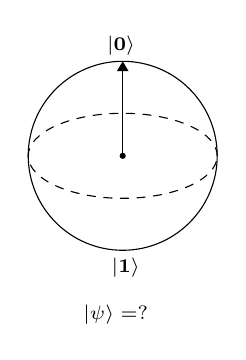
\begin{tikzpicture}[line cap=round, line join=round, >=Triangle, scale=0.6]
  \draw(0,0) circle (2cm);
  \draw [rotate around={0.:(0.,0.)},dash pattern=on 3pt off 3pt] (0,0) 
  ellipse (2cm and 0.9cm);
  \draw [->] (0,0) -- (0,2);
  \scriptsize
  \draw [fill] (0,0) circle (1.5pt);
  \draw (-0.5,2.7) node[anchor=north west] {$\mathbf {\vert 0\rangle}$};
  \draw (-0.4,-2) node[anchor=north west] {$\mathbf {\vert 1\rangle}$};
  \draw (-1,-3) node[anchor=north west] {$\vert \psi \rangle = ?$};
\end{tikzpicture} \hspace{0.5cm}

\vspace{1cm}
% make the same figure for the second state where the qubit is in the state |1>
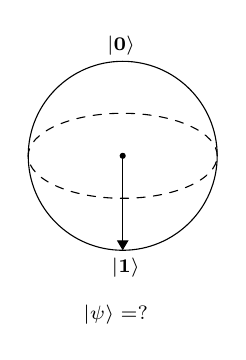
\begin{tikzpicture}[line cap=round, line join=round, >=Triangle, scale=0.6]
  \draw(0,0) circle (2cm);
  \draw [rotate around={0.:(0.,0.)},dash pattern=on 3pt off 3pt] (0,0) 
  ellipse (2cm and 0.9cm);
  \draw [->] (0,0) -- (0,-2);
  \scriptsize
  \draw [fill] (0,0) circle (1.5pt);
  \draw (-0.5,2.7) node[anchor=north west] {$\mathbf {\vert 0\rangle}$};
  \draw (-0.4,-2) node[anchor=north west] {$\mathbf {\vert 1\rangle}$};
  \draw (-1,-3) node[anchor=north west] {$\vert \psi \rangle = ?$};
\end{tikzpicture} \hspace{0.5cm}
\vspace{1cm}

% make the same figure for the third state where the qubit is in the state |+> = 1/sqrt(2) (|0> + |1>)
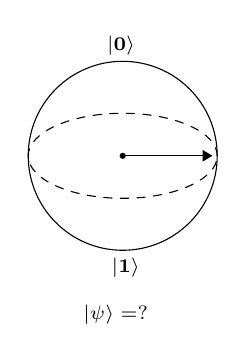
\begin{tikzpicture}[line cap=round, line join=round, >=Triangle, scale=0.6]
  \draw(0,0) circle (2cm);
  \draw [rotate around={0.:(0.,0.)},dash pattern=on 3pt off 3pt] (0,0) 
  ellipse (2cm and 0.9cm);
  \draw [->] (0,0) -- (1.9,0);
  \scriptsize
  \draw [fill] (0,0) circle (1.5pt);
  \draw (-0.5,2.7) node[anchor=north west] {$\mathbf {\vert 0\rangle}$};
  \draw (-0.4,-2) node[anchor=north west] {$\mathbf {\vert 1\rangle}$};
  \draw (-1,-3) node[anchor=north west] {$\vert \psi \rangle = ?$};
\end{tikzpicture} \hspace{0.5cm}
\vspace{1cm}

% make the same figure for the fourth state where the qubit is in the state |-> = 1/sqrt(2) (|0> - |1>)
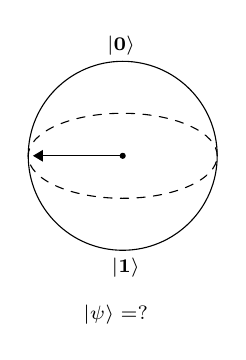
\begin{tikzpicture}[line cap=round, line join=round, >=Triangle, scale=0.6]
  \draw(0,0) circle (2cm);
  \draw [rotate around={0.:(0.,0.)},dash pattern=on 3pt off 3pt] (0,0) 
  ellipse (2cm and 0.9cm);
  \draw [->] (0,0) -- (-1.9,0);
  \scriptsize
  \draw [fill] (0,0) circle (1.5pt);
  \draw (-0.5,2.7) node[anchor=north west] {$\mathbf {\vert 0\rangle}$};
  \draw (-0.4,-2) node[anchor=north west] {$\mathbf {\vert 1\rangle}$};
  \draw (-1,-3) node[anchor=north west] {$\vert \psi \rangle = ?$};
\end{tikzpicture} \hspace{0.5cm}

\newpage 

\question {Let's emulate together a quantum circuit of two qubits 
and entangle them.}

\vspace{1cm}
We initialize both qubits in state $\ket{0}$ 
and two classical bits 
in the given quantum circuit. 
What will be the total initial state of the two qubits? \\

% draw a quantum circuit of two qubits and two classical bits?
\begin{center}
  \begin{quantikz}
    q_0 &\qw          & \qw \\
    q_1 &\qw          & \qw \\
    c_0 &\cw          & \cw \\
    c_1 &\cw          & \cw
  \end{quantikz}
\end{center}
Answer is: $\ket{q_0 q_1} = $


\vspace{3cm}
Apply a Hadamard gate to the first qubit. First, draw it in the quantum circuit given below 
and write the new state of the two qubits. \\
\vspace{3cm}  
Second, apply a CNOT gate to the two qubits. First, draw it in the quantum circuit given above
and write the new state of the two qubits. \\

\vspace{3cm}
Make your drawing here:
\begin{center}
  \begin{quantikz}
    q_0 &\qw    & \qw & \qw & \qw & \qw & \qw & \qw & \qw & \qw & \qw    & \qw \\
    q_1 &\qw    & \qw & \qw & \qw & \qw & \qw & \qw & \qw & \qw & \qw    & \qw \\
    c_0 &\cw    & \cw & \cw & \cw & \cw & \cw & \cw & \cw & \cw & \cw    & \cw \\
    c_1 &\cw    & \cw & \cw & \cw & \cw & \cw & \cw & \cw & \cw & \cw    & \cw
  \end{quantikz}
\end{center}

\newpage 


How does the state of the two qubits change after applying the Hadamard and CNOT gates? \\

\vspace{3cm}

Given the final state of the two qubits, how do you see the entanglement? \\

\newpage
\vspace{1cm}
    --------- \textit{\lastwords} ---------
    \end{center}
    
    \label{finalpage}
    \end{document}